\documentclass[border=10pt]{standalone}
\usepackage{pgfplots}
\pgfplotsset{compat=1.18}
\definecolor{myblue}{RGB}{70,110,170}
\definecolor{myorange}{RGB}{240,150,50}
\definecolor{mygreen}{RGB}{40,110,60}
\begin{document}
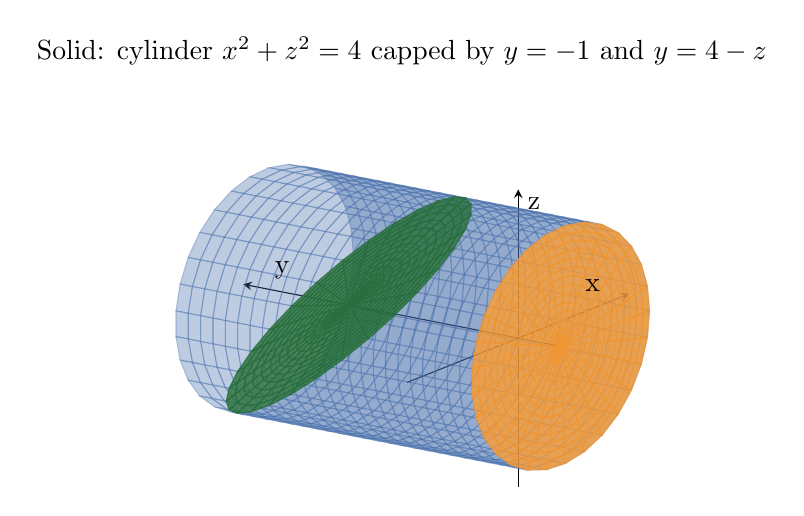
\begin{tikzpicture}
\begin{axis}[
    view={-55}{20},
    axis lines=middle,
    xlabel={x}, ylabel={y}, zlabel={z},
    xmin=-2.5, xmax=2.5, ymin=-1, ymax=6.5, zmin=-2.5, zmax=2.5,
    title={Solid: cylinder $x^2+z^2=4$ capped by $y=-1$ and $y=4-z$},
    ticks=none
]
\addplot3[surf, shader=flat, opacity=0.35, color=myblue,
    domain=0:360, y domain=-1:6, samples=30, samples y=25]
({2*cos(x)}, {y}, {2*sin(x)});
\addplot3[surf, shader=flat, opacity=0.8, color=myorange,
    domain=0:360, y domain=0:2, samples=30, samples y=15]
({y*cos(x)}, {-1}, {y*sin(x)});
\addplot3[surf, shader=flat, opacity=0.8, color=mygreen,
    domain=0:360, y domain=0:2, samples=30, samples y=15]
({y*cos(x)}, {4 - y*sin(x)}, {y*sin(x)});
\end{axis}
\end{tikzpicture}
\end{document}